\documentclass[conference]{IEEEtran}
\usepackage[utf8]{inputenc}
\usepackage[T1]{fontenc}
\usepackage[ngerman]{babel}
\usepackage[autostyle=true]{csquotes}
\usepackage{graphicx}
\graphicspath{{../00_Bilder/}{../Quellen_PDF/}}
\usepackage{siunitx}
\sisetup{locale = DE}
\usepackage{cite}
\usepackage[justification=raggedright, singlelinecheck=false]{caption}

\begin{document}

\title{Entwicklung Digitaler Zwillinge für Lehrzwecke am Beispiel Maze~Runner und Dobot~Magician mit NVIDIA~Omniverse}

\author{
\IEEEauthorblockN{Tobias Küster}
\IEEEauthorblockA{
Hochschule Hannover -- University of Applied Sciences and Arts\\
Fakultät II -- Maschinenbau und Bioverfahrenstechnik\\
Labor für Produktentwicklung und Digitale Fabrik\\
tobias.kuester1@gmail.com}
}

\maketitle

\begin{abstract}
In der digitalisierten Fabrikplanung gelten Digitale Zwillinge als Bindeglied zwischen physischer Anlage und virtuellem Modell.
Diese Arbeit untersucht Potenziale und Herausforderungen Digitaler Zwillinge mittels NVIDIA~Isaac~Sim.
Im Labor für Produktentwicklung und Digitale Fabrik (LFP) der Hochschule Hannover wurden dazu für zwei reale Anlagen, den Rundtakttisch \enquote{Maze~Runner} und den Desktoproboter \enquote{Dobot~Magician}, Digitale Zwillinge entwickelt und in Betrieb genommen.
Der Maze~Runner wurde über OPC~UA und MQTT, der Dobot~Magician über die Python-Bibliothek \emph{pydobot} bidirektional an NVIDIA~Isaac~Sim gekoppelt.
Ergänzend entstand eine methodische Reproduzierbarkeitsdokumentation im PowerPoint-Foliensatz-Format für den Nachbau beider Digitalen Zwillinge.
Aus den Ergebnissen werden branchenübergreifende Potenziale sowie sieben konkrete Handlungsempfehlungen für das LFP abgeleitet.
\end{abstract}

\begin{IEEEkeywords}
Digitale Zwillinge, NVIDIA Omniverse, NVIDIA Isaac Sim, OpenUSD, Fabrikplanung, virtuelle Inbetriebnahme, OPC UA, pydobot, MQTT
\end{IEEEkeywords}

\section{Einleitung}
Die produzierende Industrie steht unter dem Druck kürzerer Innovationszyklen, steigender Variantenvielfalt und zunehmenden Verdrängungswettbewerbs.
Industrie-4.0-Lösungsansätze bieten dem deutschen Maschinen- und Anlagenbau die Möglichkeit, auf diese Herausforderungen zu reagieren und durch Digitalisierung und Vernetzung neue Geschäftsmodelle zu erschließen, wie Abbildung~\ref{fig:dt_manufacturing} darstellt~\cite{plattformi40_fortschrittsbericht2024,kagermann2013}.
Moderne Simulationsplattformen wie NVIDIA~Omniverse fassen dazu Modelldaten unterschiedlicher Planungswerkzeuge in einer gemeinsamen Echtzeitsimulation zusammen und stellen Anlage und Produkt fotorealistisch sowie physikalisch korrekt dar~\cite{nvidia_omniverse,bmw_nvidia_2021}.
Für den Einsatz als Digitaler Zwilling reicht ein geometrisches Modell allein jedoch nicht aus, die Komponenten müssen zusätzlich über eine bidirektionale Kommunikationsanbindung mit realen Anlagensignalen verknüpft werden~\cite{kritzinger2018}.
Da NVIDIA~Omniverse keine eigene Anbindungslogik für die beiden Anlagen mitbringt, ist für jede Anlage die Entwicklung einer eigenen Extension erforderlich, die das geometrische Modell in der NVIDIA-Isaac-Sim-Oberfläche bidirektional an die reale Anlage koppelt und die Kommunikation mit der realen Steuerung übernimmt.
Abbildung~\ref{fig:mazerunner_extension} zeigt exemplarisch einen der beiden im Rahmen dieser Arbeit entstandenen Digitalen Zwillinge in NVIDIA~Isaac~Sim.

\begin{figure}[t]
\centering
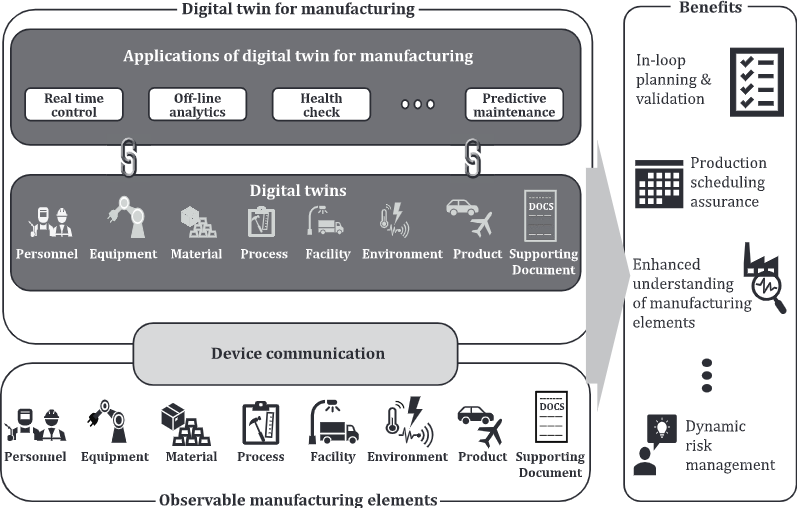
\includegraphics[width=0.92\linewidth]{05_IoT_Rahmenwerk_ISO23247-1_Zusammenfassung}
\caption{Übersicht Digitaler Zwillinge in der produzierenden Industrie und deren Vorteile (Quelle: ISO/FDIS~23247-1~\cite{iso23247}, Figure~2).}
\label{fig:dt_manufacturing}
\end{figure}

Ziel dieser Arbeit ist es, Potenziale und Herausforderungen der Integration Digitaler Zwillinge in die Fabrikplanung mit NVIDIA~Isaac~Sim systematisch zu untersuchen.
Dazu wurden im Labor für Produktentwicklung und Digitale Fabrik (LFP) der Hochschule Hannover Digitale Zwillinge zweier grundverschiedener Anlagen entwickelt, erprobt und dokumentiert.
Der Maze~Runner ist eine Rundtaktanlage, deren speicherprogrammierbare Steuerung (SPS) logische Ein- und Ausgänge als Datengrundlage bereitstellt.
Der Dobot~Magician ist dagegen ein Gelenkarmroboter, der über Gelenkwinkel angesteuert wird, wodurch im digitalen Modell eine grundlegend andere kinematische Architektur entsteht.
Beide Anlagen unterscheiden sich in Aufbau, Kommunikationsprotokoll und Modellierungsansatz, um die Übertragbarkeit der entwickelten Methodik auf unterschiedliche Anlagentypen zu prüfen.
Wie weit jede der beiden Anlagen dabei tatsächlich zu einem vollwertigen Digitalen Zwilling wird, lässt sich erst anhand eines geeigneten Reifegradmodells beurteilen.

\begin{figure}[t]
\centering
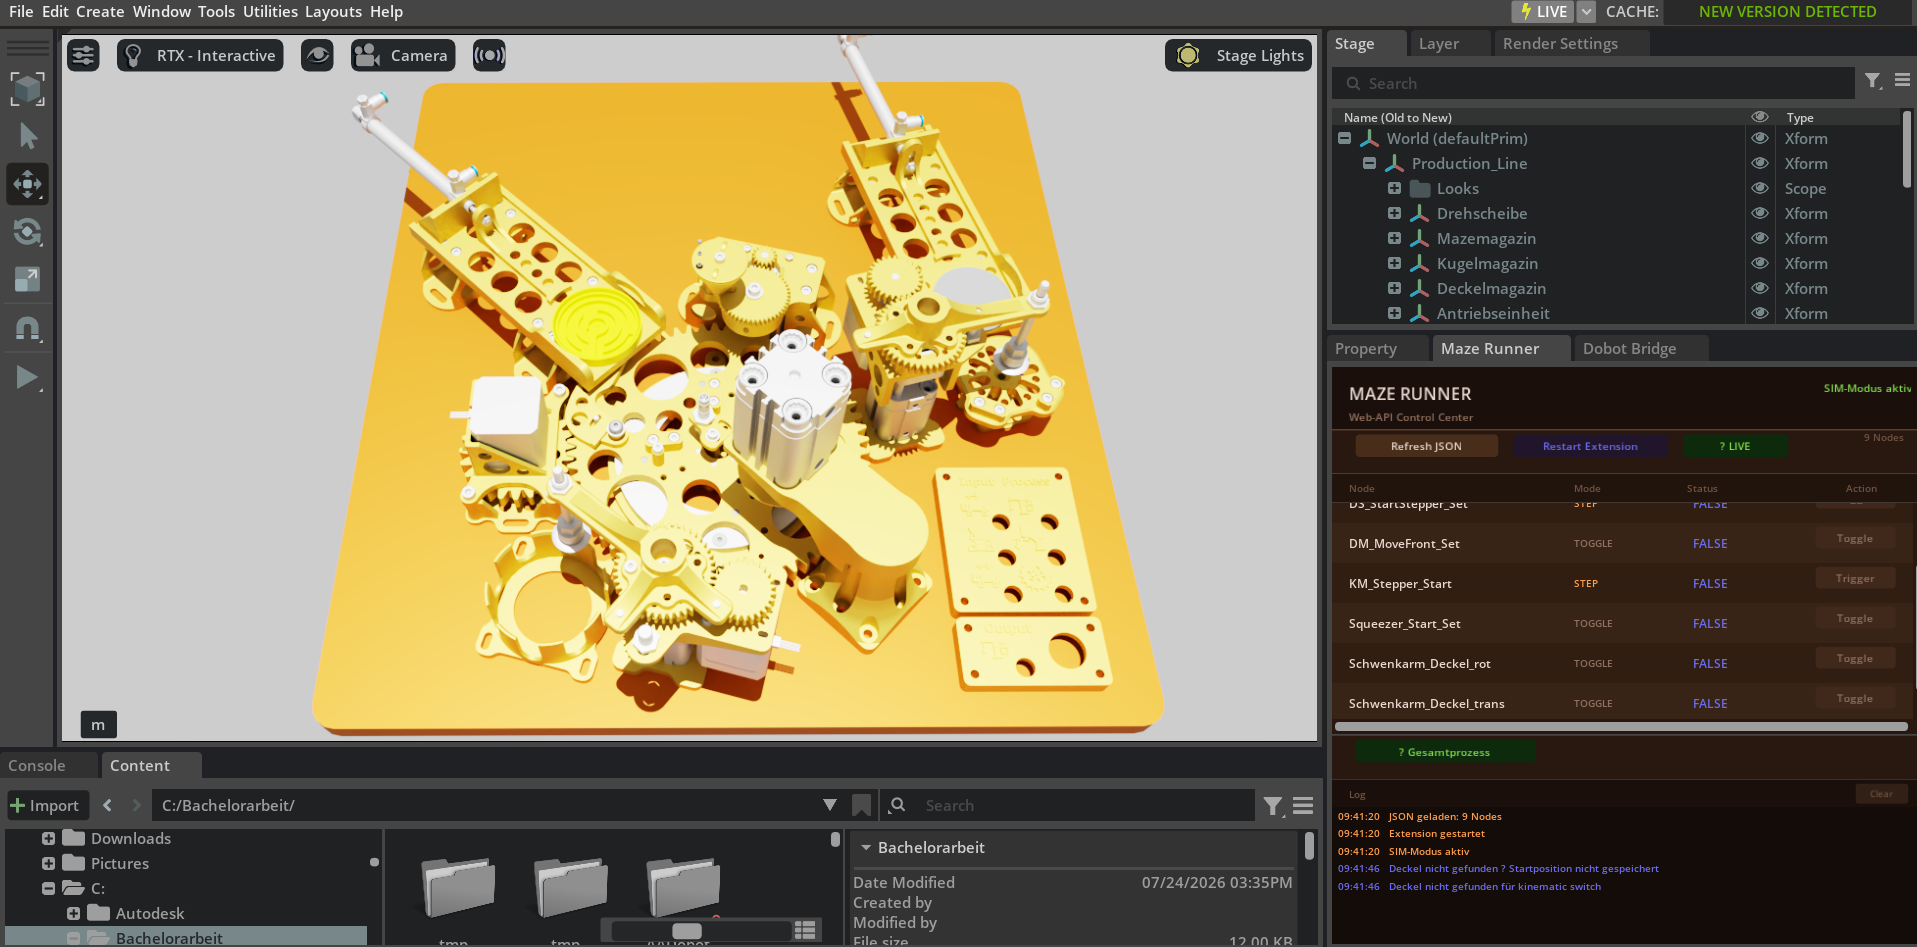
\includegraphics[width=0.92\linewidth]{22_Benutzeroberflaeche_Mazerunner_Extension}
\caption{Digitaler Zwilling der Maze-Runner-Anlage in NVIDIA Isaac Sim mit eingeschaltetem, angedocktem HMI (Eigene Darstellung).}
\label{fig:mazerunner_extension}
\end{figure}

\section{Theoretischer Rahmen (Kurzüberblick)}
Um den erreichten Kopplungsgrad beider Anlagen im weiteren Verlauf einheitlich einordnen zu können, wird zunächst eine begriffliche Abgrenzung Digitaler Zwillinge benötigt, wofür zwei sich ergänzende Rahmenwerke herangezogen werden.
Nach Kritzinger et al.\ lässt sich anhand des Datenflusses zwischen realer Anlage und virtuellem Modell unterscheiden, ob überhaupt ein Digitaler Zwilling vorliegt, wie Abbildung~\ref{fig:kritzinger_klassifikation} anhand der Reifegrade \emph{Digitales Modell}, \emph{Digitaler Schatten} und \emph{Digitaler Zwilling} zeigt~\cite{kritzinger2018}.

\begin{figure}[h]
\centering
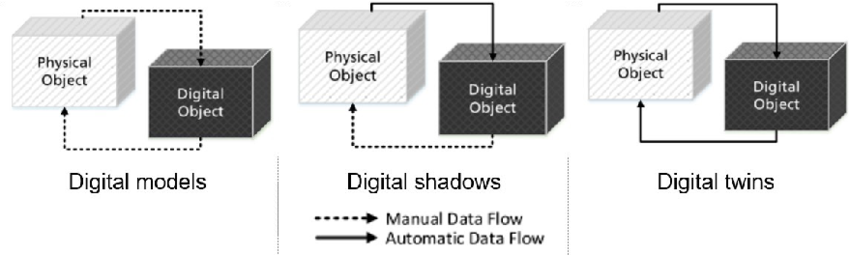
\includegraphics[width=0.9\linewidth]{03_Kritzinger_Klassifikation_Digitaler_Zwilling}
\caption{Datenfluss im Digitalen Modell, im Digitalen Schatten und im Digitalen Zwilling (Quelle: \cite{kritzinger2018}).}
\label{fig:kritzinger_klassifikation}
\end{figure}

Ergänzend zu dieser Schwellenwertbetrachtung beschreibt das Reifegradmodell von Shao et al.\ den Funktionsumfang eines Digitalen Zwillings, von der reinen Beobachtung bis zur eigenständigen Korrektur durch einen intelligenten Digitalen Zwilling, wie Abbildung~\ref{fig:shao_reifegrad} zeigt~\cite{shao2023standardized}.

\begin{figure}[h]
\centering
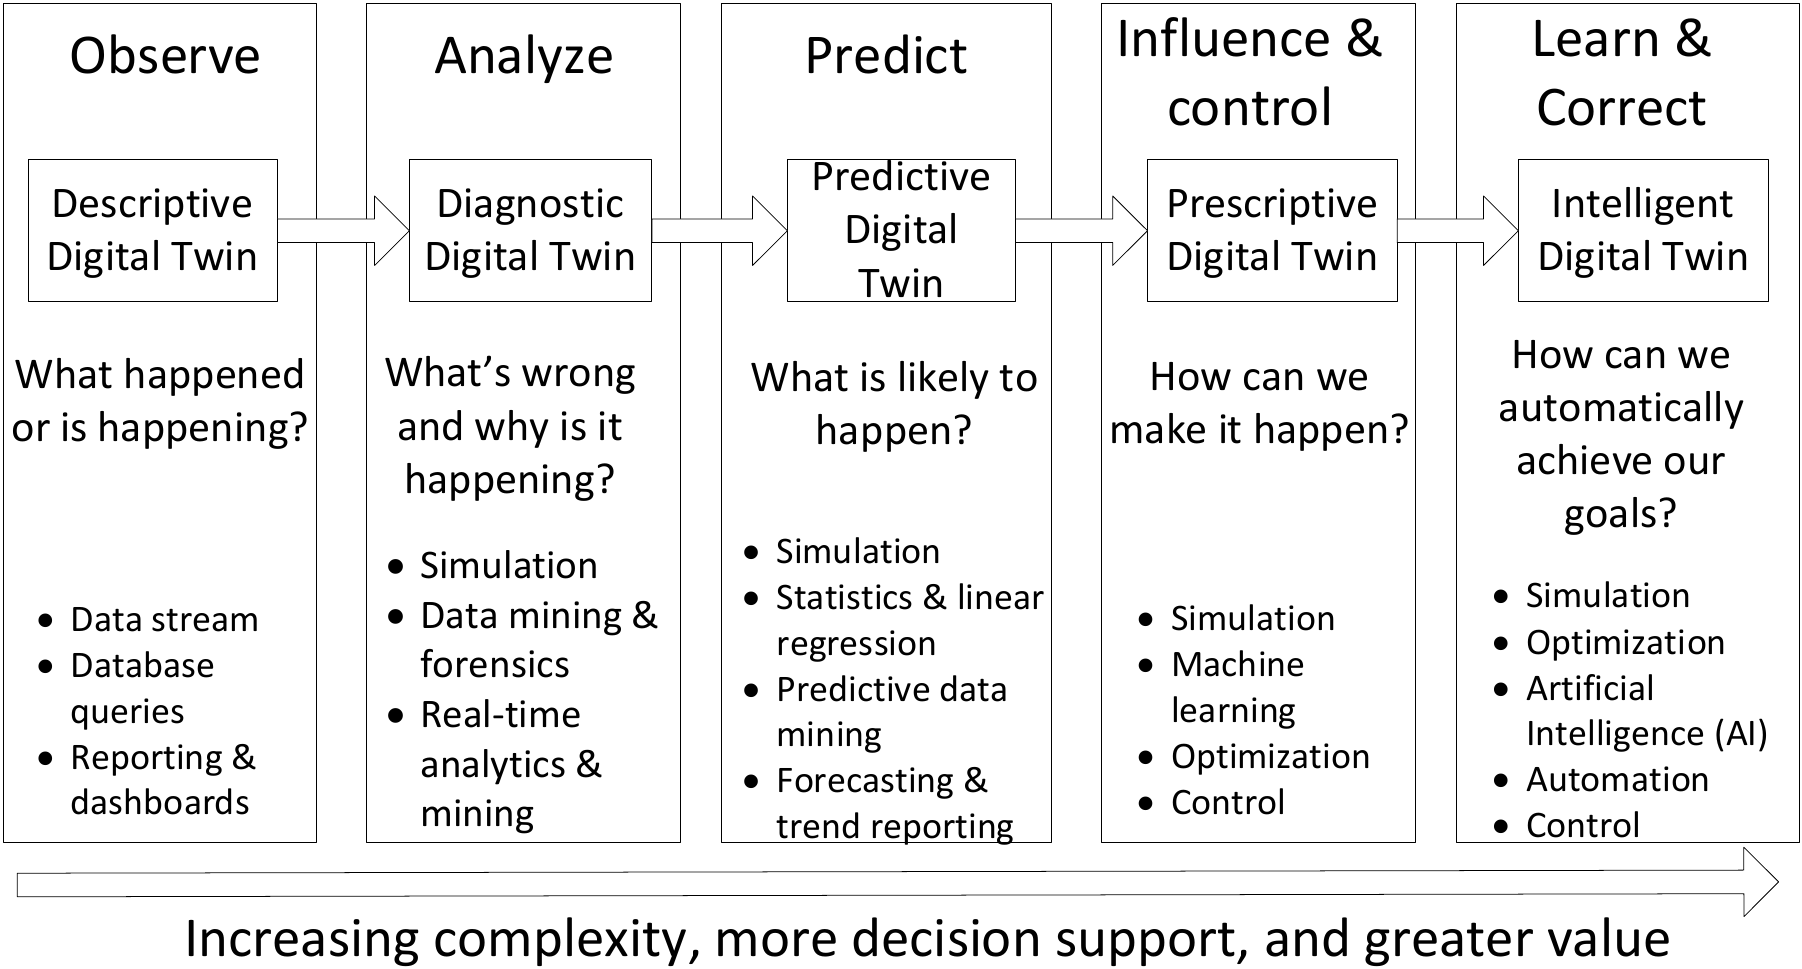
\includegraphics[width=0.9\linewidth]{04_Shao_Reifegradmodell_Digitaler_Zwilling}
\caption{Reifegradmodell Digitaler Zwillinge nach Funktionsumfang, von der Beobachtung bis zur eigenständigen Korrektur (Quelle: \cite{shao2023standardized}).}
\label{fig:shao_reifegrad}
\end{figure}

Diese beiden Einordnungen bilden gemeinsam den Maßstab, an dem sich die beiden im Folgenden vorgestellten Digitalen Zwillinge messen lassen.
Weitere theoretische Grundlagen zum Digital-Twin-Framework nach ISO~23247, zum Referenzarchitekturmodell RAMI~4.0~\cite{plattformi40_rami40_orientierungsrahmen} sowie zu den Datenformaten OpenUSD und URDF sind der vollständigen Bachelorarbeit zu entnehmen.

\section{Digitaler Zwilling: Maze Runner}
Der Maze~Runner ist ein Rundtakttisch mit acht Stationen, darunter Boden- und Deckelmagazin, Pufferstation, Presse und Ausgabeschwenkarm, dessen Ablauf über eine Siemens-SPS~S7-1200 gesteuert wird.
Das gefertigte Produkt besteht dabei aus Labyrinth (Boden), Metallkugel und Plexiglasplatte, wie Abbildung~\ref{fig:aktorik_produkt} zeigt.
Die Anlage wurde von Herrn Yübo~Wang an der Hochschule~RheinMain (HSRM) für die industrielle Automatisierungslehre entwickelt und wird dort im Rahmen einer hochschulübergreifenden Vorlesung eingesetzt, an der internationale Partnerhochschulen wechselseitig auf die Digitalen Zwillinge der beteiligten Standorte zugreifen~\cite{wang2024mazerunner}.
Im Zuge einer Hochschulkooperation mit der HSRM wurde der Maze~Runner an das LFP der Hochschule~Hannover übergeben, in Betrieb genommen und im Rahmen der vorliegenden Arbeit um den beschriebenen Digitalen Zwilling ergänzt.

\begin{figure}[!t]
\centering
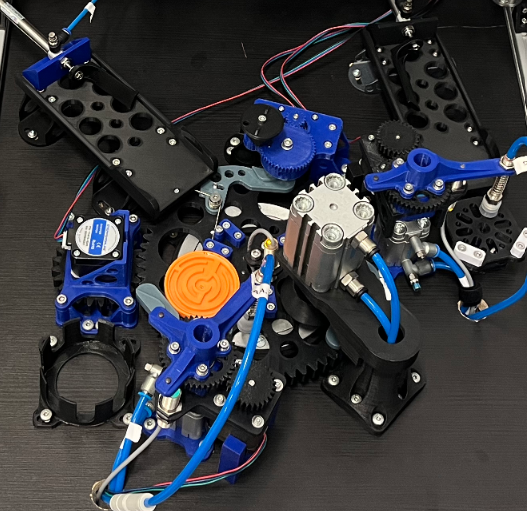
\includegraphics[height=4.8cm]{15_Aktorik_Mazerunner_Anlage}\hspace{0.3cm}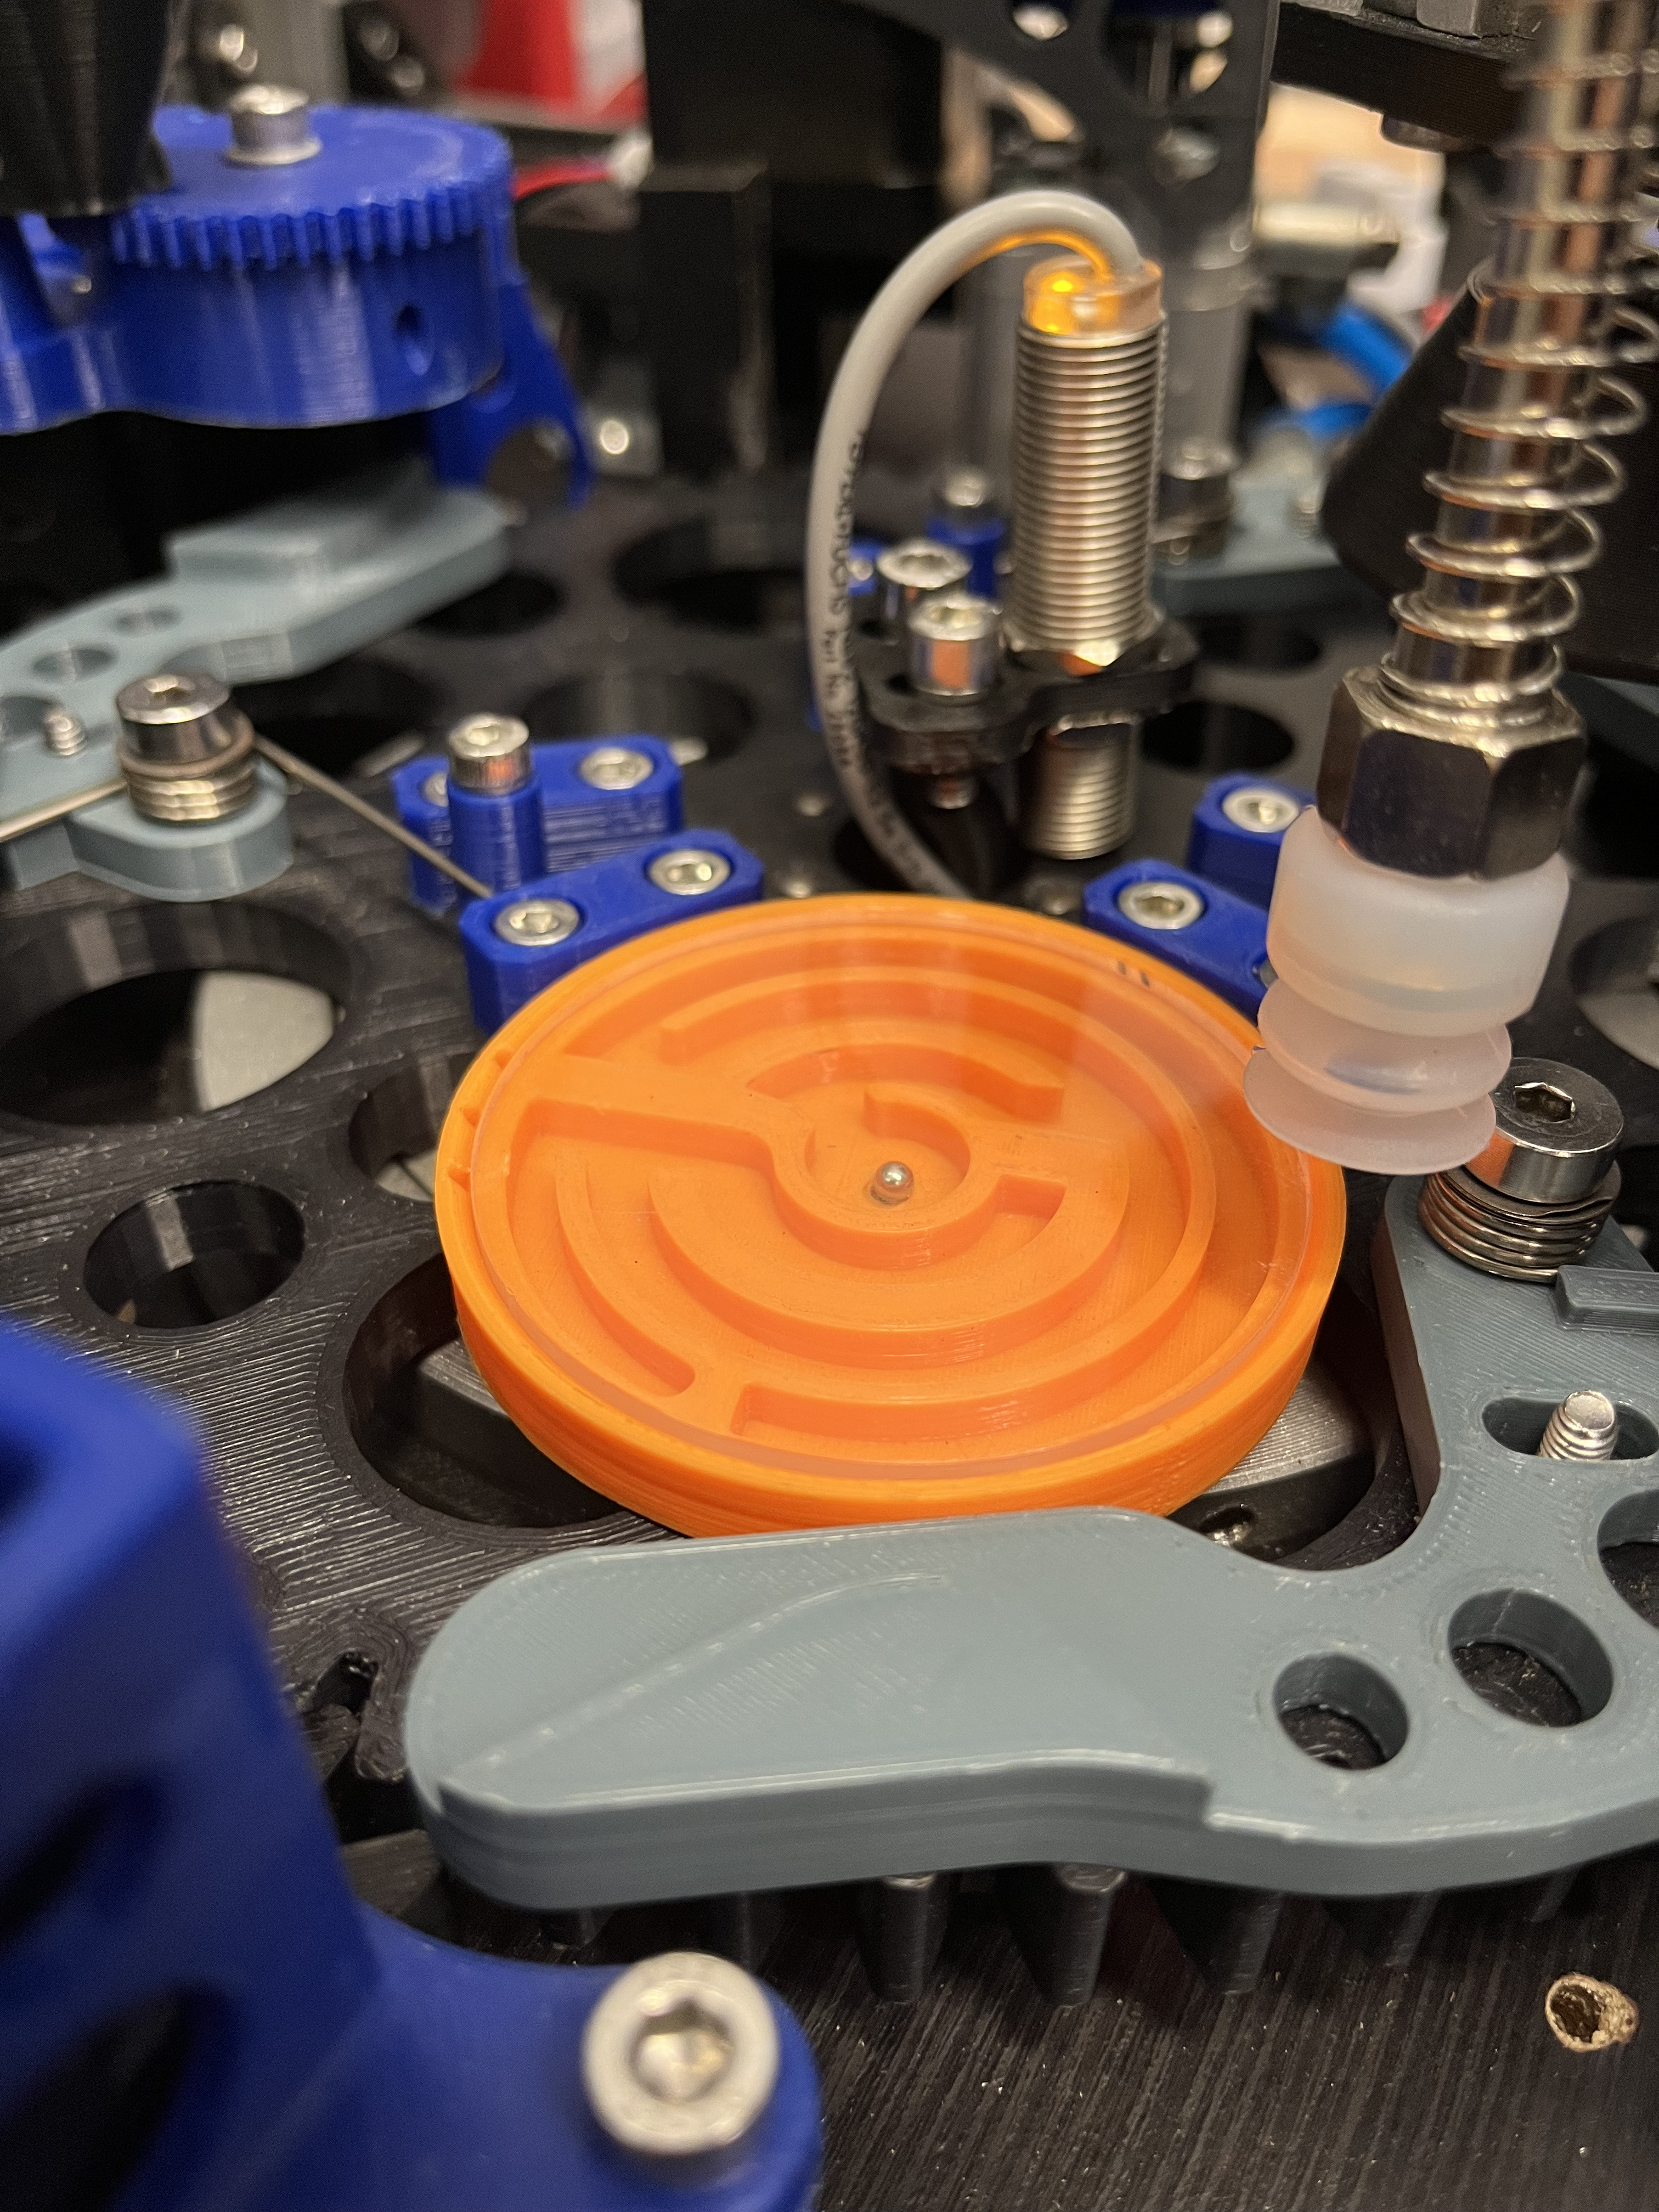
\includegraphics[height=4.8cm]{16_Produkt_Mazerunner_Drehscheibe}
\caption{Aktorik der Maze-Runner-Anlage (links) und gefertigtes Produkt auf der Drehscheibe (rechts) (Eigene Aufnahme).}
\label{fig:aktorik_produkt}
\end{figure}

Das vom Kooperationspartner bereitgestellte CAD-Modell wird über den Isaac-Sim-STEP-Importer nach OpenUSD überführt, die Kinematik durch PhysX-\emph{Articulations} abgebildet.
Die SPS-Signale werden als OPC-UA-Knoten bereitgestellt und über eine zwölf Python-Module umfassende Extension sowie den \emph{DigitalTwinService} der HSRM per REST-API und MQTT an die Simulation gekoppelt, wobei die datengetriebene Konfiguration über \texttt{nodes\_db.json} die Übertragung auf weitere SPS-gestützte Anlagen ohne tiefgreifende Quellcodeänderungen ermöglicht.
Der vollständige Steuerpfad erreicht dabei zuverlässig eine Latenz zwischen \SI{100}{\milli\second} und \SI{500}{\milli\second}, während sich die Rückmeldung der Sensorwerte über MQTT im Laborbetrieb nicht durchgängig zuverlässig erwies.
Die realisierte Kopplung entspricht daher eher einer erweiterten Fernsteuerung (Teleoperation) als einem vollständig bidirektionalen Digitalen Zwilling nach Kritzinger et al.

\begin{figure*}[t]
\centering
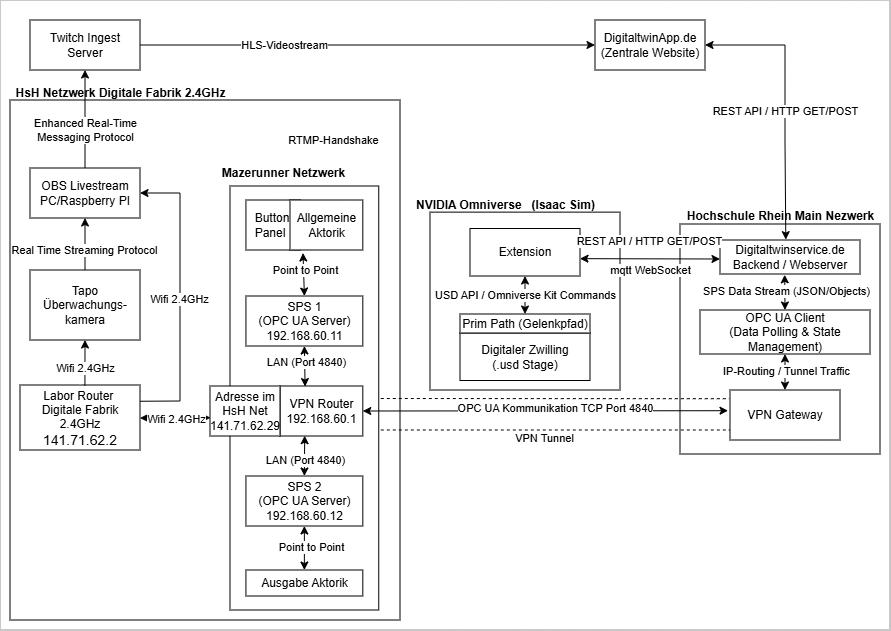
\includegraphics[width=0.85\textwidth]{27_Netzwerkarchitektur_DigitalTwinApp_HSRM}
\caption{Netzwerkarchitektur zur Anbindung Digitaler Zwillinge in NVIDIA Omniverse an die Digital Twin App der HSRM, mit den drei Netzwerkzonen Labor, HSRM und freiem Internet (Eigene Darstellung nach HSRM-Dokumentation~\cite{wang2024mazerunner}).}
\label{fig:mazerunner_ibd}
\end{figure*}

\section{Digitaler Zwilling: Dobot Magician}
Neben der SPS-gestützten Rundtaktanlage des Maze~Runners entstand im Rahmen dieser Arbeit mit dem Dobot~Magician ein zweiter, kinematisch grundlegend andersartiger Digitaler Zwilling.
Der vierachsige Desktop-Roboterarm erhielt dabei ein eigenständiges Pick-and-Place-Szenario, in dem eine Schutzkappe auf ein Modellfahrzeug des DeLorean aus \enquote{Zurück in die Zukunft} aufgesetzt wird, wie in Abbildung~\ref{fig:dobot_dt} rechts im Digitalen und links im realen Aufbau im LFP gezeigt wird.

\begin{figure}[h]
\centering
\begin{minipage}[t]{0.48\linewidth}
\centering
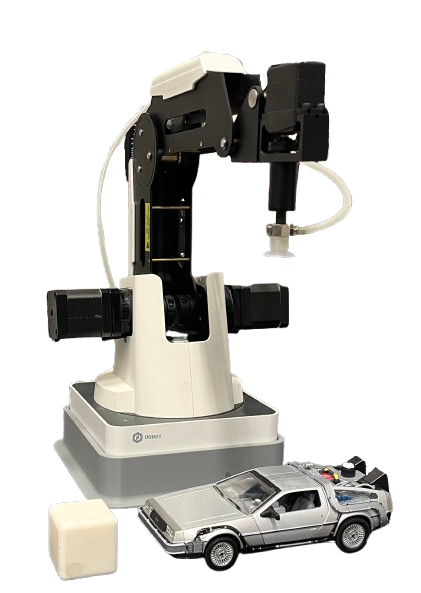
\includegraphics[width=\linewidth]{34_PnP_Szenario_LFP}
\end{minipage}
\hfill
\begin{minipage}[t]{0.48\linewidth}
\centering
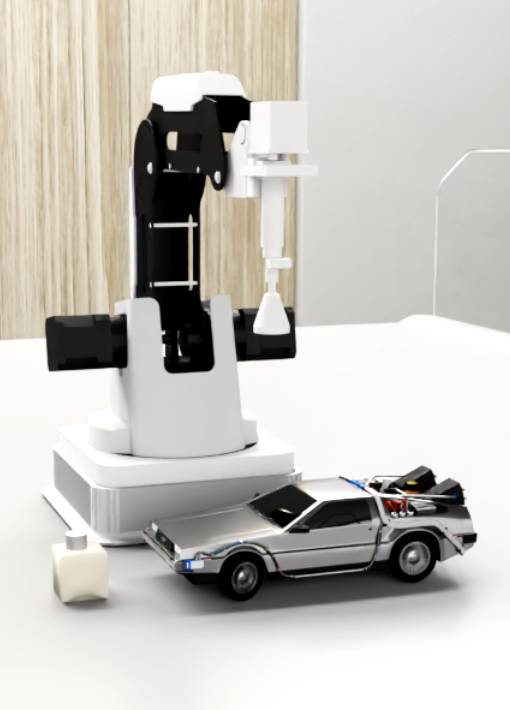
\includegraphics[width=\linewidth]{33_PnP_Szenario_IsaacSim}
\end{minipage}
\caption{Pick-and-Place-Szenario des Dobot Magician real im LFP (links) und als Digitaler Zwilling in NVIDIA Isaac Sim (rechts) (Eigene Aufnahme/Darstellung).}
\label{fig:dobot_dt}
\end{figure}

Er kommuniziert ausschließlich seriell über UART mittels USB-Port, wofür die Extension \texttt{Dobot\_DT\_IsaacSim\_Extension} die Python-Bibliothek \emph{pydobot} nutzt, um zyklisch die reale Pose auszulesen und die berechneten Gelenkwinkel über die Dynamic-Control-API von NVIDIA~Isaac~Sim auf die per URDF-Import geladene Articulation des Robotermodells zu schreiben, wobei das kinematisch geschlossene Parallelogrammgetriebe des Unterarms nicht im URDF-Modell nachgebildet, sondern rechnerisch kompensiert wird.

Über das Bedienpanel lassen sich Jog-, Vertikal- und Sauggreifer-Befehle direkt an den realen Roboterarm senden, zudem lassen sich vollständige Pick-and-Place-Sequenzen per Teach-In am physischen Roboter aufzeichnen und automatisiert wiedergeben.
Mit dem automatisierten Datenfluss zur Simulation erreicht der Dobot~Magician die Stufe des Digitalen Schattens und ergänzt diesen um eine manuell auslösbare Fernsteuerung in Gegenrichtung, realisiert über eine feste Namenskonvention, mit \texttt{sim\_} beginnende Methoden wirken auf die Simulation, mit \texttt{real\_} beginnende Methoden auf den realen Dobot~Magician.

\begin{figure}[!t]
\centering
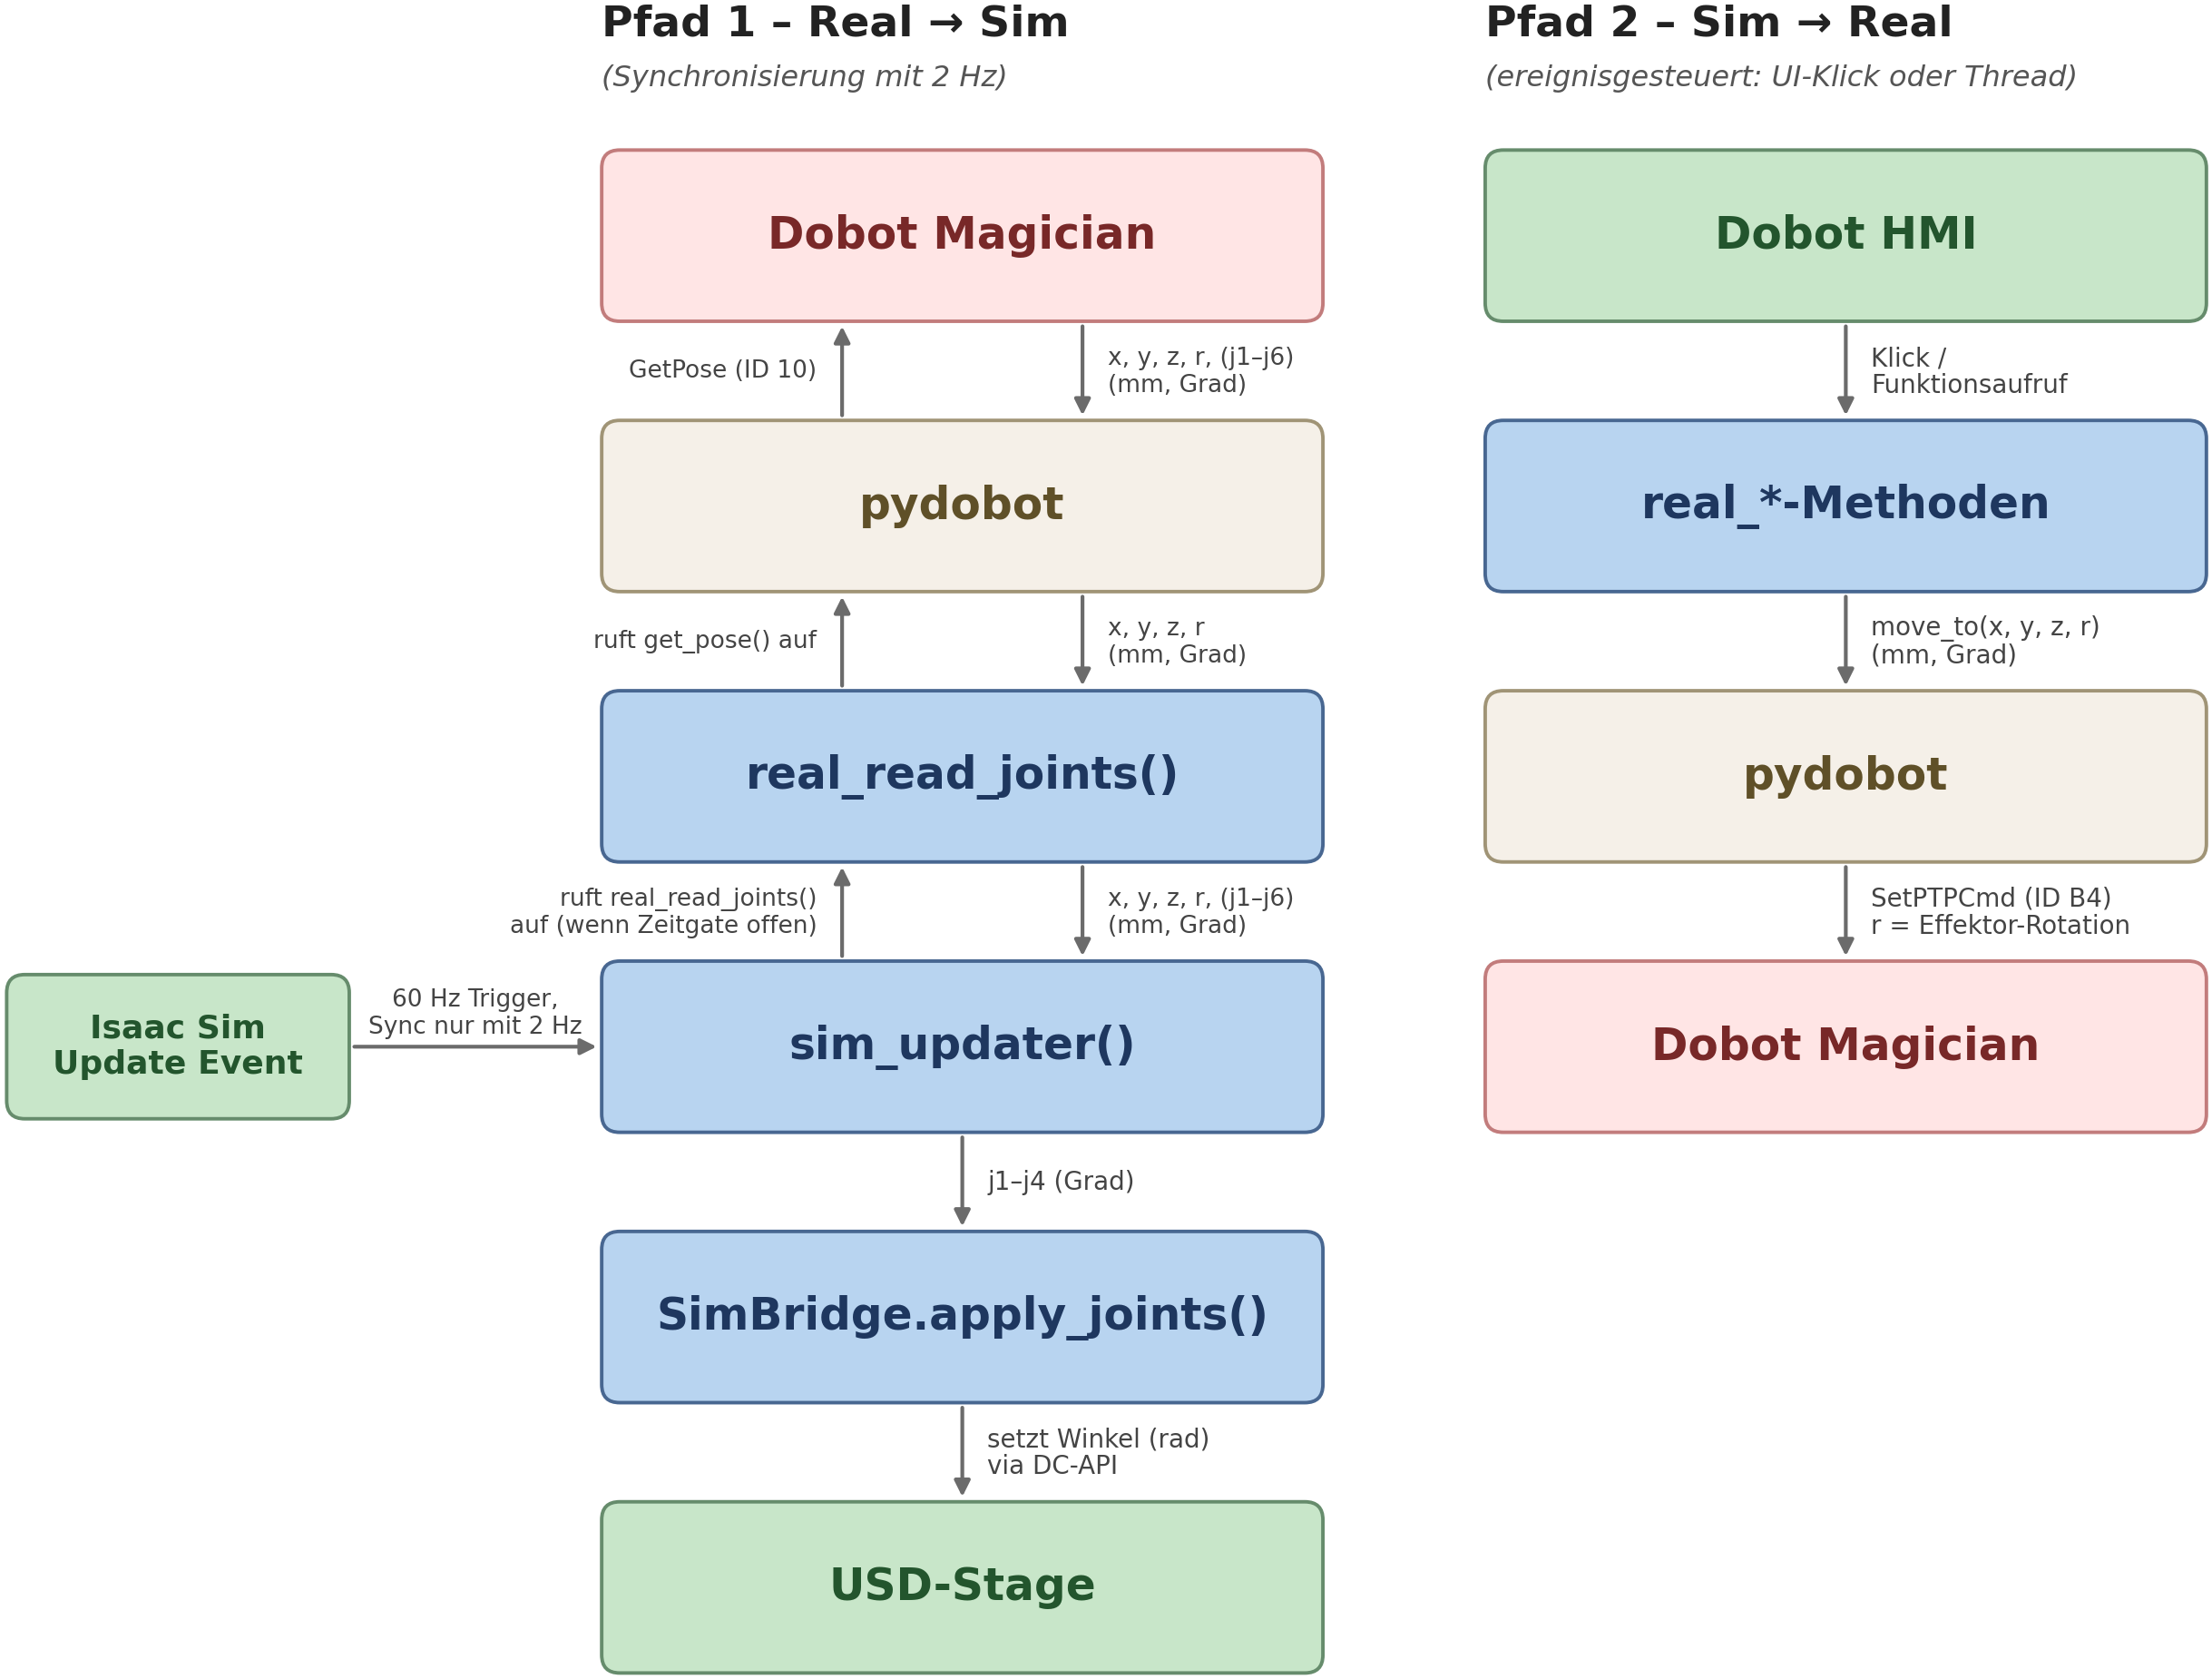
\includegraphics[width=\linewidth]{40_Datenflussstruktur_Dobot_Extension}
\caption{Datenflussstruktur der Dobot-Magician-Extension zwischen realem Dobot Magician und NVIDIA Isaac Sim (Eigene Darstellung).}
\label{fig:dobot_wege}
\end{figure}

\section{Validierung und Ergebnisse}
Für beide Anlagen wurde eine methodische Reproduzierbarkeitsdokumentation als Schritt-für-Schritt-Anleitung im PowerPoint-Foliensatz erstellt, die jeweils zusätzlich als PDF-Datei vorliegt und sich damit auch für den Einsatz in der Lehre eignet.
Beide wurden von mehreren Personen unabhängig durchlaufen und validiert, ihre Ergebnisse flossen in die jeweilige Anleitung zurück.
Eine ergänzend über die in NVIDIA Isaac Sim integrierte OpenXR-Schnittstelle erprobte VR-Anwendung auf der Meta~Quest~3 erwies sich als nicht vollständig funktionsfähig, da sich keine echtzeitfähige Übertragung des Modells feststellen ließ, was der Grafik- und Prozessorleistung der eingesetzten Hardware zuzuschreiben sein könnte.
Aus den Ergebnissen wurden vier zentrale Nutzungspotenziale abgeleitet, darunter virtuelle Inbetriebnahme (VIBN) neuer Steuerungsprogramme, Kollisionsüberwachung durch Abgleich realer und virtueller Trajektorien, datengetriebene Erweiterbarkeit der Extension-Architektur auf weitere SPS-gestützte Anlagen ohne Quellcodeänderungen sowie synthetische Datengenerierung fotorealistischer Trainingsbilder für KI-gestützte Greifpunktdetektion.
Hinsichtlich der Skalierbarkeit wächst die GPU-Last dabei linear mit der Anzahl gleichzeitig simulierter Articulations, weshalb der gleichzeitige Betrieb beider Digitalen Zwillinge auf einer leistungsfähigeren Workstation geprüft werden sollte, bevor weitere Anlagen ergänzt werden.
Beide Extensions sowie die zugehörigen USD-Stages wurden gemäß Aufgabenstellung digital an das LFP übergeben.

Die Inbetriebnahme und Weiterentwicklung der Maze-Runner-Anlage erfolgte in enger Abstimmung mit Herrn~Yübo~Wang, der im zweiwöchigen Rhythmus über Microsoft Teams Anforderungen besprach und diese in einem Kanban-Board in Jira festhielt, darunter eine bereits erprobte, jedoch noch nicht hinreichend zuverlässige Flexibilisierungsschablone mit Dobot-Einsatz, die die im Ausblick beschriebene engere Verknüpfung beider Anlagen bereits im Entwicklungsprozess vorwegnimmt.

\section{Diskussion}
Beide Anlagen erreichen nach Kritzinger et al.\ einen unterschiedlichen Kopplungsgrad.
Der Dobot~Magician realisiert einen vollständigen Digitalen Schatten, ergänzt um eine manuell auslösbare Fernsteuerung in Gegenrichtung, während der Maze~Runner aufgrund der nicht durchgängig zuverlässigen MQTT-Rückmeldung eher einer erweiterten Teleoperation entspricht als einem vollständig bidirektionalen Digitalen Zwilling.
Diese Differenz lässt sich auf die unterschiedliche Middleware-Architektur zurückführen, die dreistufige Kopplung über \emph{DigitalTwinService}, VPN-Tunnel und OPC-UA beim Maze~Runner bietet zwar Ortsunabhängigkeit und Mehrbenutzerfähigkeit für die hochschulübergreifende Vorlesung, erkauft dies jedoch mit zusätzlicher Netzwerklatenz und potenziellen Störquellen gegenüber der direkten seriellen USB-Kopplung des Dobot~Magician über \emph{pydobot}.
Für Anlagen mit vergleichbaren Anforderungen an Fernzugriff und Mehrbenutzerbetrieb ist die aufwändigere Architektur des Maze~Runners daher trotz der genannten Einschränkungen die zweckmäßigere Wahl, während sich die schlanke pydobot-Kopplung für lokal betriebene Einzelarbeitsplätze empfiehlt.
Beide Extensions teilen sich dennoch eine gemeinsame methodische Grundlage aus Anforderungsanalyse, Import in NVIDIA Isaac Sim, Kinematikdefinition und Kopplung an die reale Anlage, wodurch sich die entwickelte Vorgehensweise trotz unterschiedlicher Protokolle grundsätzlich auf weitere Anlagentypen übertragen lässt.
Einschränkend zu nennen sind die am Dobot~Magician nicht modellierte geschlossene kinematische Kette des Parallelogrammgetriebes sowie die fehlende Greifer-Rückmeldung, die beide die Simulationsgenauigkeit zugunsten einer vereinfachten, für den Digitalen Schatten hinreichenden Modellierung begrenzen.
Für den Dobot~Magician hat sich das als Industriestandard geltende ROS~2 im Rahmen dieser Arbeit als unnötig komplex herausgestellt, während die Einfachheit von \emph{pydobot} einem geringeren Vorwissen in der Programmierung entgegenkommt.
Für vergleichbare Laboraufbauten empfiehlt sich daher eine Kombination beider Ansätze, OPC~UA und MQTT auf Anlagenebene sowie pydobot auf Roboterebene, wobei die Zuverlässigkeit der jeweiligen Rückmeldekanäle vor einer produktiven Nutzung gesondert zu prüfen ist.
Der Betrieb von NVIDIA~Isaac~Sim setzt zudem eine RTX-fähige GPU mit ausreichender Rechenleistung voraus, für die gesamte Entwicklung diente durchgängig ein Laptop mit einer NVIDIA~RTX~4070-Laptop-GPU und einem Intel~Core~i7-13620H, dessen Leistung für einen einzelnen Digitalen Zwilling ausreichte.
Beim Betrieb eines Digitalen Zwillings stieß die Hardware jedoch an ihre Grenzen, sobald zusätzlich ein weiterer Dienst im Hintergrund aktiv war, was die entsprechende Handlungsempfehlung zur Beschaffung einer leistungsfähigeren Workstation begründet.

\section{Potenziale und Handlungsempfehlungen}
Über die im vorigen Abschnitt diskutierten anlagenspezifischen Erkenntnisse hinaus bieten Digitale Zwillinge nach ISO~23247-1 auch branchenübergreifende Potenziale, darunter vorausschauende Planung und Validierung von Produktionsabläufen, eine verlässlichere Produktionsplanung, ein vertieftes Verständnis der beteiligten Fertigungselemente sowie dynamisches Risikomanagement~\cite{iso23247}.
Diese Potenziale erschließen sich jedoch nur, wenn Digitale Zwillinge nicht als kundenspezifische Einzellösung entstehen, sondern auf einem einheitlichen Rahmen aufbauen~\cite{shao2023standardized}.
Ein weiterer branchenweiter Vorteil ergibt sich aus der Standardisierung über die Asset Administration Shell der IDTA, die Maschinendaten wie Simulationsmodelle in strukturierten Submodellen ablegt und dadurch deren Weitergabe an einen neuen Betreiber ermöglicht, etwa beim Verkauf einer Maschine oder Komponente~\cite{zhang2025aas}.
Diesen Potenzialen steht am LFP die Herausforderung gegenüber, dass die Weiterführung der Extensions bislang von einzelnen Personen mit entsprechender Zusatzqualifikation in OpenUSD, Python-Scripting, OPC~UA und MQTT abhängt, eine Kombination, die in klassischen Maschinenbau-Curricula bislang selten gemeinsam vertreten ist, weshalb ein Ausscheiden dieser Personen ohne strukturierte Übergabe einen Verlust an implizitem Wissen über die Extensions riskiert.
Für das LFP werden daraus sieben konkrete Handlungsempfehlungen abgeleitet.
\begin{enumerate}
\item Fertigstellung des Maze~Runners durch Klärung der unregelmäßigen MQTT-Rückmeldungen gemeinsam mit den IT-Verantwortlichen der HSRM, um Anlage und Digitalen Zwilling vollständig zusammenzuführen,
\item Beschaffung einer leistungsfähigeren Workstation, um NVIDIA Isaac Sim unter Höchstlast zu prüfen und den gleichzeitigen Betrieb beider Digitalen Zwillinge zu erproben,
\item Automatisierung der Dobot-Fernsteuerung durch Verfolgen eines virtuellen Zielwürfels, wodurch die Richtung der Fernsteuerung anschaulich demonstriert wird,
\item Übertragung der Reproduzierbarkeitsdokumentation auf weitere Laboranlagen und Roboterarme im LFP, etwa den vorhandenen UR3-Roboterarm oder den KUKA-KR6-Roboterarm, wobei die Ergebnisse dieser Arbeit den Aufwand je Anlage erheblich reduzieren,
\item Vertiefung von Omniverse-Anwendungen in der Lehre anhand der von NVIDIA bereitgestellten, sechsteiligen Robot-Setup-Tutorial-Reihe (vgl.\ Abbildung~\ref{fig:ur10_tutorial}), die ohne Programmiererfahrung durchführbar ist~\cite{nvidia_isaacsim_manipulator_tutorial},
\item Ausbau der Kooperation mit der HSRM im Rahmen der dortigen globalen Vorlesung sowie Aufbau von Informatik-Expertise im LFP, um die Betreuung stärker auf Maschinenbau-Fragestellungen auszurichten,
\item Erwerb von Lizenzen für IDE-integrierte KI-Werkzeuge zur Unterstützung der Softwareentwicklung, alternativ bei zu hoher Komplexität grafische Offline-Programmiersoftware wie KUKA.Sim.
\end{enumerate}

\begin{figure}[t]
\centering
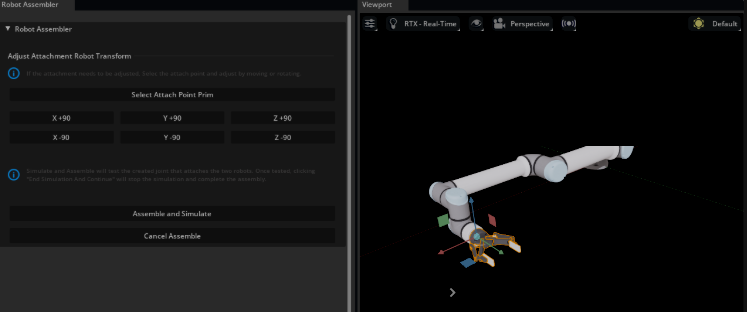
\includegraphics[width=0.92\linewidth]{42_Tutorial_UR10_Assemblierung_RobotAssembler}
\caption{NVIDIA-Isaac-Sim-Tutorial zur Assemblierung eines UR10-Manipulators mit Robotiq-2F-140-Greifer über den Robot Assembler, übertragbar auf den im LFP vorhandenen UR3-Roboterarm mit Robotiq-2F-140-Greifer~\cite{nvidia_isaacsim_manipulator_tutorial}.}
\label{fig:ur10_tutorial}
\end{figure}

\section{Fazit und Ausblick}
\subsection{Zentrale Erkenntnisse}
Die vorliegende Arbeit hat gezeigt, dass sich Digitale Zwillinge auch für grundverschiedene Anlagentypen, eine SPS-gestützte Fertigungslinie und einen seriell angesteuerten Gelenkarmroboter, mit einer gemeinsamen Simulationsplattform realisieren lassen, wobei sich der jeweils erreichte Kopplungsgrad deutlich unterscheidet.
Das bereits einleitend neben Kritzinger et al.\ vorgestellte Reifegradmodell von Shao et al.\ ordnet die umgesetzte Pick-and-Place-Anwendung des Dobot~Magician als deskriptiven Digitalen Zwilling ein, wie Abbildung~\ref{fig:shao_reifegrad} zeigt, da die Echtzeitübertragung der Gelenkwinkel in die Simulation lediglich der Beobachtung des aktuellen Anlagenzustands dient, ohne Abweichungen zu bewerten oder Handlungen abzuleiten~\cite{shao2023standardized}.
Die Wahl der Middleware sollte sich dabei stets am tatsächlichen Vernetzungsbedarf der Anlage orientieren, die aufwändigere, mehrbenutzerfähige Architektur des Maze~Runners eignet sich für ortsunabhängigen Fernzugriff, während die schlanke pydobot-Kopplung des Dobot~Magician für lokal betriebene Einzelarbeitsplätze die einfachere und robustere Wahl darstellt.
Da alle Disziplinen von Mechanik über Steuerungstechnik bis zur Softwareentwicklung durch eine Einzelperson zu bearbeiten waren, zeigt die Arbeit zudem, dass sich eine an VDI~2221~\cite{vdi_konstruktionsmethodik} orientierte, disziplinübergreifende Vorgehensweise auch für komplexe mechatronische Digitalisierungsvorhaben eignet, sofern ausreichend Zeit für die Einarbeitung in die beteiligten Werkzeuge eingeplant wird.
Die für beide Anlagen dokumentierten Arbeitsschritte, von der Anforderungsanalyse über den Import in NVIDIA Isaac Sim bis zur Kopplung an die reale Steuerung, könnten künftig einem KI-System als Spezifikation dienen, anhand derer sich Digitale Zwillinge automatisiert erstellen und schrittweise bis zu einem intelligenten Digitalen Zwilling nach dem Funktionsumfang von Shao et al.\ weiterentwickeln lassen~\cite{shao2023standardized}.

\subsection{Ausblick}
Für den Maze~Runner stehen zunächst die Fertigstellung der Anlage durch Klärung der unregelmäßigen MQTT-Rückmeldungen sowie die Weitervermittlung des erlangten Wissens im Rahmen der globalen Vorlesung von Herrn Wang im Vordergrund, ergänzend könnten kürzere Pneumatikzylinder die vorerst nicht verbauten Turmmagazine reaktivieren und eine Serienproduktion ermöglichen.
Für den Dobot~Magician sollte die Extension um weitere Bedienelemente erweitert und für komplexere, mehrstufige Pick-and-Place-Aufgaben ausgelegt werden, etwa das Schließen der DeLorean-Tür.
Der Dobot~Magician selbst verfügt neben dem verwendeten Sauggreifer über weitere Endeffektoren wie einen mechanischen Greifer, der sich möglicherweise mit demselben Isaac-Sim-Werkzeug zur Assemblierung von Manipulatoren erproben ließe.
Der Sauggreifer selbst wird zwar über das HMI ferngesteuert, sein Zustand wird jedoch bislang weder ausgelesen noch in der Stage abgebildet, da die in Abbildung~\ref{fig:gelenkwinkel} dargestellte Extension ausschließlich die Gelenkwinkel J1 bis J3 in Echtzeit ausliest.
Ein neuer Greifer müsste daher, ebenso wie das Ansaugen selbst, über ein Fixed Joint dargestellt werden, das die Oberfläche des Sauggreifers mit der Oberfläche der Schutzkappe verbindet, sobald innerhalb eines bestimmten Koordinatenfeldes angesaugt wird.

\begin{figure}[t]
\centering
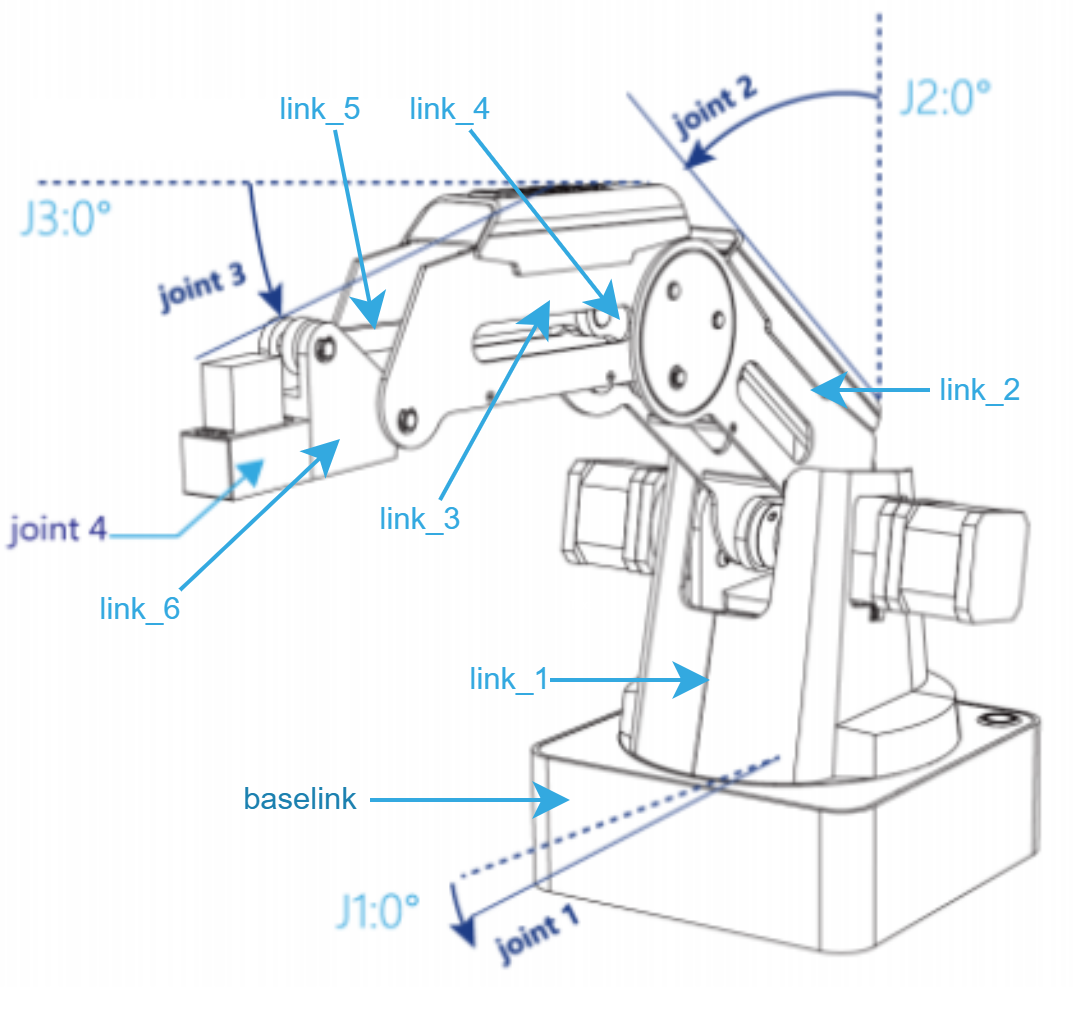
\includegraphics[width=0.68\linewidth]{35_Gelenkwinkelkonvention_Dobot_J1_J4}
\caption{Gelenkwinkelkonvention des Dobot Magician mit den vier Gelenken J1 bis J4, von denen die Extension J1 bis J3 in Echtzeit ausliest (Eigene Darstellung nach Dobot Robotics~\cite{dobot_magician}).}
\label{fig:gelenkwinkel}
\end{figure}
Über den Dobot~Magician hinaus erscheint zudem die Erprobung weiterer, im LFP vorhandener Manipulatoren vielversprechend, da sich das genutzte NVIDIA-Tutorial zu Import und Assemblierung von Manipulatoren grundsätzlich auf andere Robotermodelle übertragen lässt, wobei zwischen dem Dobot~Magician und den im Tutorial verwendeten Universal-Robots-Manipulatoren klar zu unterscheiden ist, da die dort gezeigten Greifer speziell für diese Baureihe ausgelegt sind~\cite{nvidia_isaacsim_manipulator_tutorial}.
Beide Anlagen könnten zudem stärker miteinander verknüpft werden, indem die Pick-and-Place-Anwendung des Dobot~Magician die Ausgabestation des Maze~Runners ersetzt und beide Digitalen Zwillinge in einer gemeinsamen Omniverse-Stage vereint werden, wofür erste Vorarbeiten in Form einer noch nicht hinreichend zuverlässigen Flexibilisierungsschablone bereits während der Anlagenweiterentwicklung entstanden sind.
Durch eine ergänzende Analysefunktion, etwa zur Erkennung einer ausbleibenden oder dysfunktionalen Sauggreifer-Funktion, ließe sich der Dobot-Digitale-Zwilling zudem von der deskriptiven auf eine diagnostische Stufe nach Shao et al.\ heben.
Mit Blick auf die eingangs vorgestellten Reifegrade nach Kritzinger et al.\ und Shao et al.\ bildet bereits ein Digitaler Schatten wie beim Dobot~Magician einen belastbaren Ausgangspunkt für spätere KI-gestützte Erweiterungen bis hin zum intelligenten Digitalen Zwilling, ohne dass die Architektur der Extension dafür grundlegend verändert werden müsste.
Ergänzend bietet sich für das LFP die Erprobung weiterer Omniverse-Instanzen an, etwa Isaac~Lab für das Training von Regelungsstrategien, Isaac~GR00T für den im LFP vorhandenen humanoiden Roboter sowie Isaac~TeleOp für die Fernsteuerung, wodurch sich das erworbene Wissen über NVIDIA~Isaac~Sim über die beiden hier entwickelten Digitalen Zwillinge hinaus nutzen ließe.
Da die HsH voraussichtlich als einzige an der globalen Vorlesung beteiligte Hochschule bereits die Grundlage zur Kopplung von Dobot~Magician und Maze~Runner gelegt hat, könnte sie nach deren Fertigstellung in diesem Themenbereich eine Vorreiterrolle einnehmen und dabei auf die Unterstützung der übrigen Hochschulen aus dem Verbund der HSRM zurückgreifen.
Über die hier behandelte Ebene der Fertigungsanlage und des Gelenkarmroboters hinaus ließe sich das Konzept des Digitalen Zwillings zudem auf eine tiefere Ebene anwenden und dem Produktentwicklungsaspekt des LFP dienen, etwa indem einzelne im Labor konstruierte Bauteile selbst als Digitale Zwillinge abgebildet werden, wodurch für die Lehre stets ein greifbares Gegenstück zur theoretischen Auseinandersetzung entstünde.
Damit liefert diese Arbeit für das LFP nicht nur zwei funktionsfähige Digitale Zwillinge, sondern auch eine methodische Grundlage, auf der sich weitere Digitalisierungsvorhaben in Fabrikplanung und Produktentwicklung gleichermaßen aufbauen lassen.

\section*{Danksagung}
Der Autor dankt Prof.\,Dr.-Ing.\,P.\,Diersen für die Betreuung der zugrunde liegenden Bachelorarbeit sowie Herrn Yübo~Wang (Hochschule~RheinMain) für die Bereitstellung und Unterstützung bei der Maze-Runner-Anlage.

\begin{thebibliography}{00}
\bibitem{kritzinger2018} W.~Kritzinger \emph{et al.}, IFAC PapersOnLine, 2018.
\bibitem{iso23247} ISO/FDIS 23247-1, 2021.
\bibitem{shao2023standardized} G.~Shao \emph{et al.}, NIST, 2023.
\bibitem{nvidia_omniverse} NVIDIA Corporation, 2025.
\bibitem{bmw_nvidia_2021} BMW Group, 2021.
\bibitem{nvidia_isaacsim_manipulator_tutorial} NVIDIA Corporation, 2025.
\bibitem{plattformi40_fortschrittsbericht2024} Plattform Industrie 4.0, 2025.
\bibitem{kagermann2013} H.~Kagermann \emph{et al.}, acatech, 2013.
\bibitem{plattformi40_rami40_orientierungsrahmen} Plattform Industrie 4.0 und ZVEI, 2024.
\bibitem{vdi_konstruktionsmethodik} VDI Zentrum Ressourceneffizienz, 2017.
\bibitem{wang2024mazerunner} X.~Wang und Y.~Wang, Hochschule RheinMain, 2024.
\bibitem{zhang2025aas} J.~Zhang \emph{et al.}, Software and Systems Modeling, 2025.
\bibitem{dobot_magician} Dobot Robotics Co., Ltd., 2023.
\end{thebibliography}

\end{document}
